%https://www.integral-domain.org/lwilliams/Resources/TikzImg/uniformtilings.tex
\documentclass[tikz]{standalone}

\definecolor{hexcolor}{RGB}{217,230,232}  %grey
\definecolor{dodecolor}{RGB}{227,203,29}   % yellow
\definecolor{squarecolor}{RGB}{119,190,175}  % light teal
\definecolor{tricolor}{RGB}{208,77,37}  % red

\begin{document}
    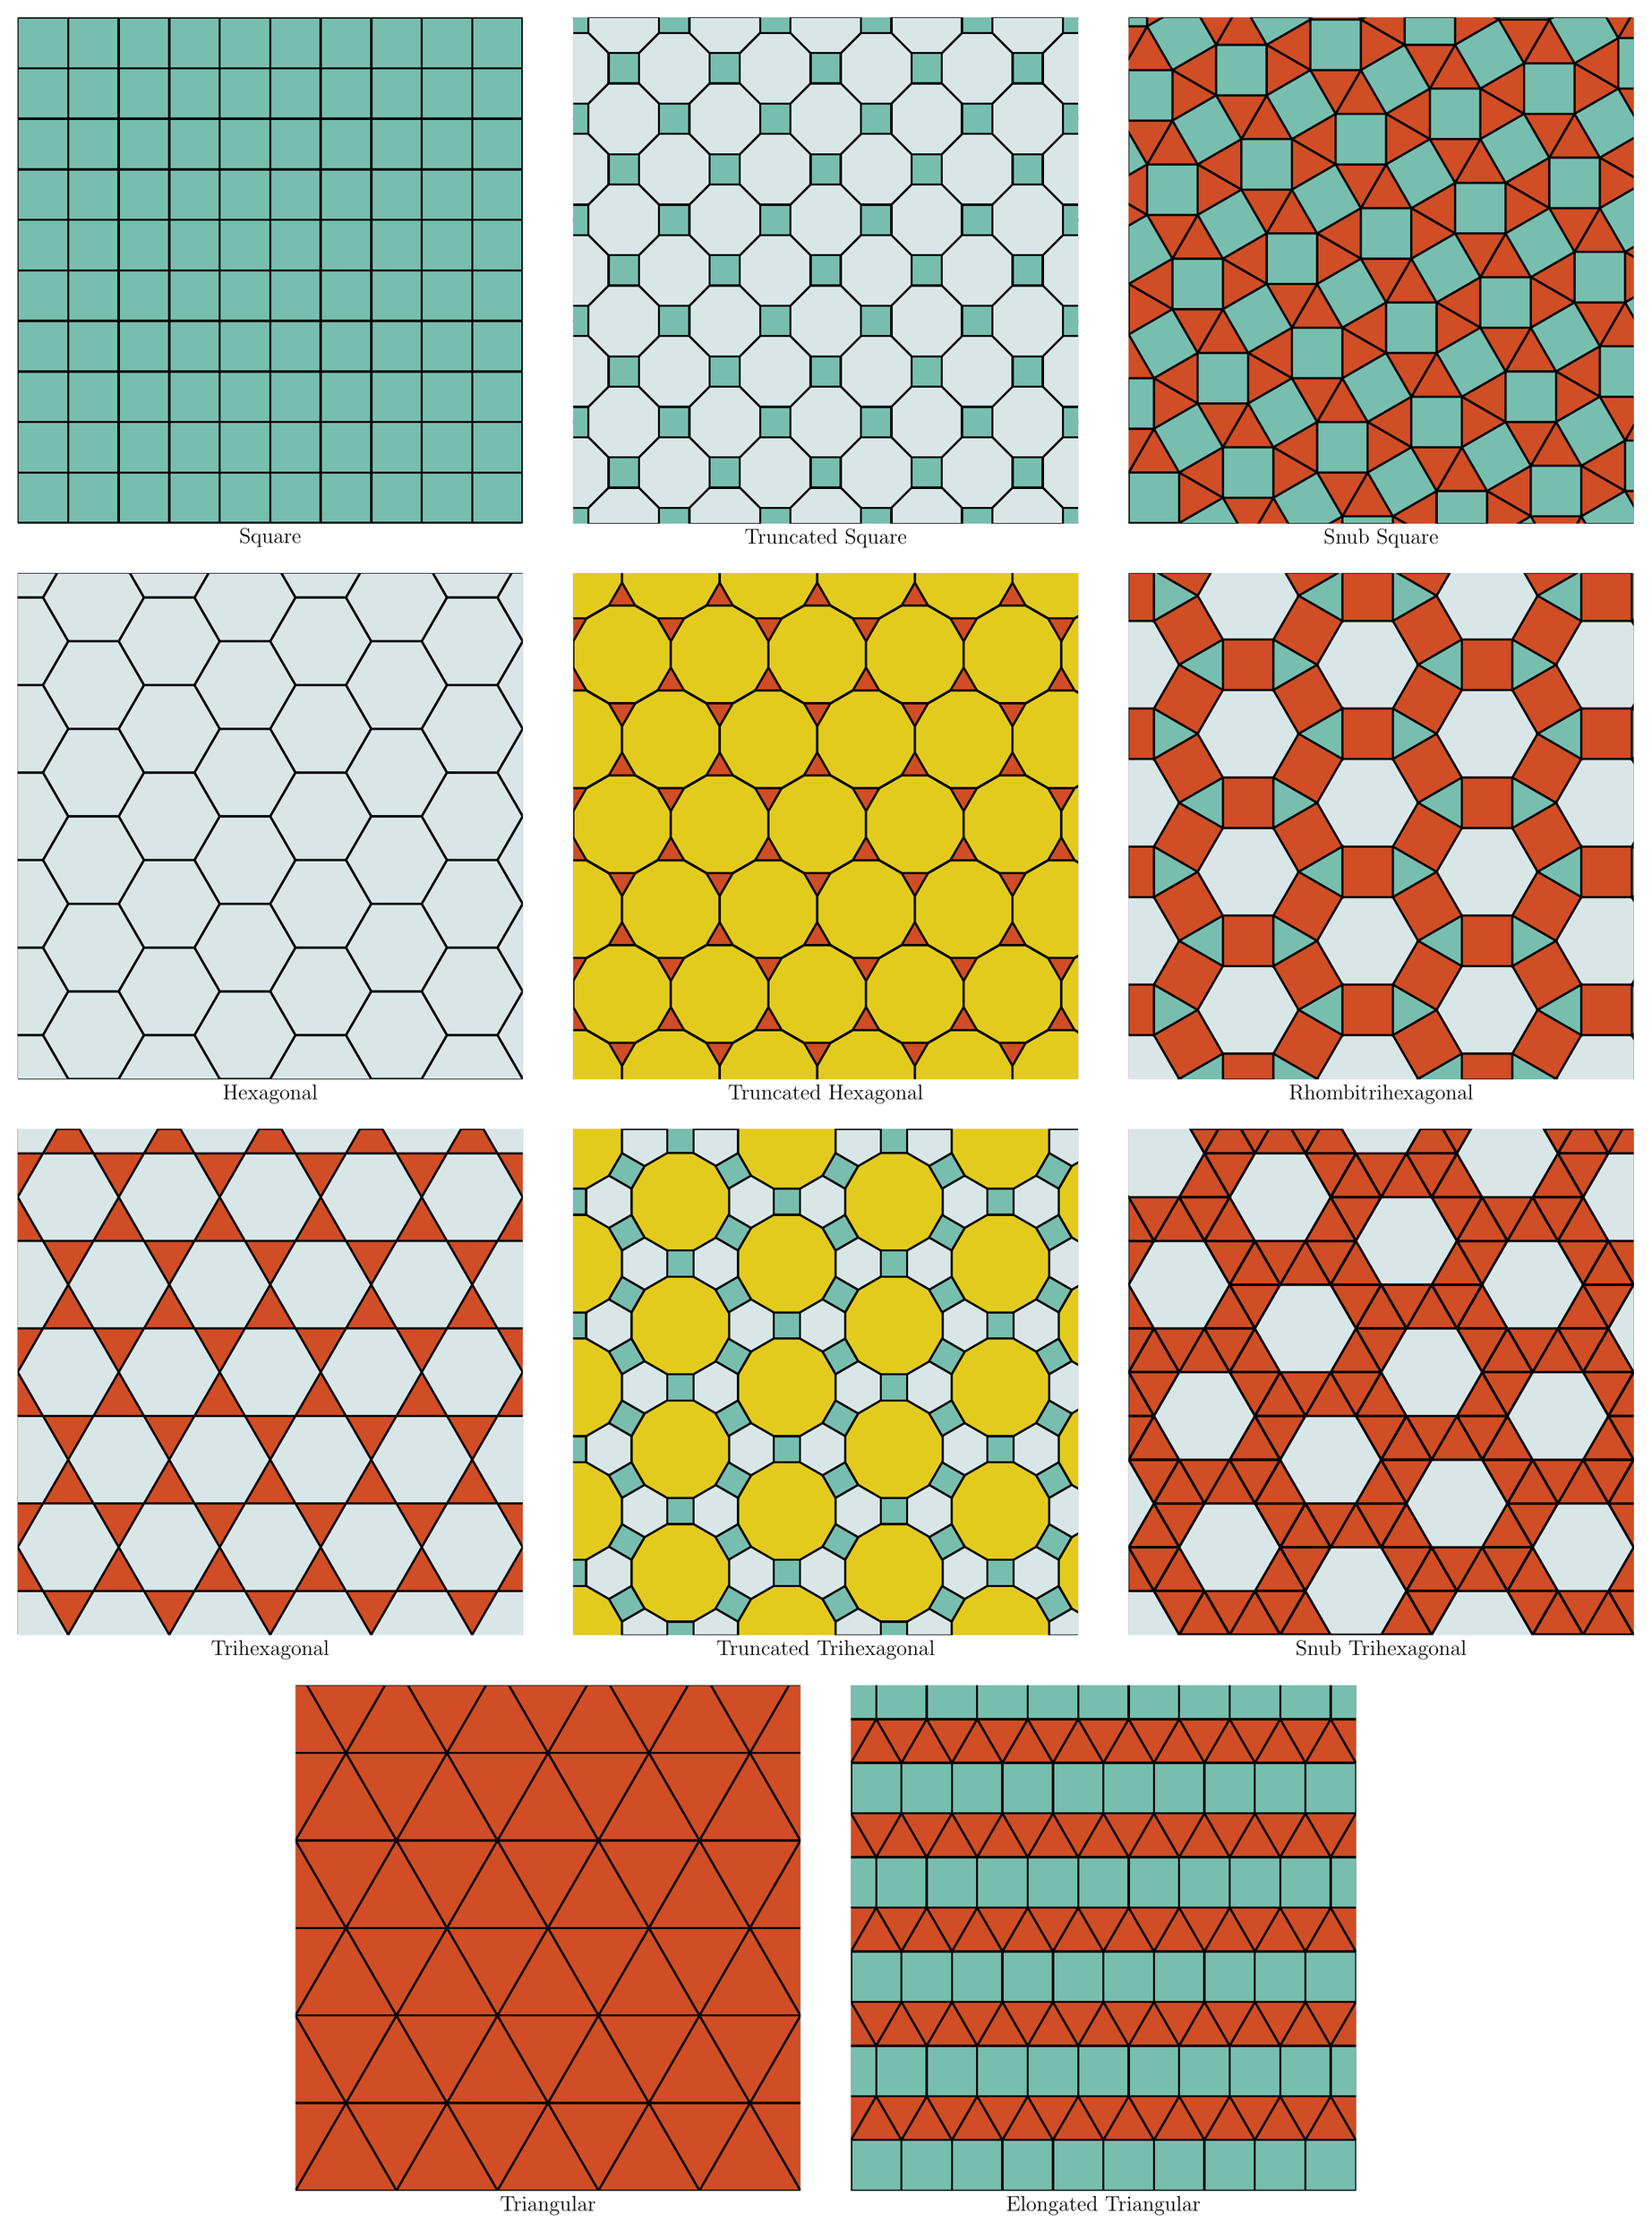
\begin{tikzpicture}[scale=1]

    \begin{scope}

        \clip (0,0)--(10,0)--(10,10)--(0,10)--(0,0);
        \draw[fill=squarecolor] (0,0)--(10,0)--(10,10)--(0,10)--(0,0);

        \draw[very thick] (0,0) grid (10,10);
    \end{scope}
    \node at (5,-0.3) {\large Square};


    \begin{scope}[xshift=11cm]

        \clip (0,0)--(10,0)--(10,10)--(0,10)--(0,0);
        \draw[fill=hexcolor] (0,0)--(10,0)--(10,10)--(0,10)--(0,0);

        \foreach \x in {-5,-4,-3,-2,-1,0,1,2,3,4}{
        \begin{scope}[xshift = \x*2 cm]
            \draw[very thick](0,0)--(12,12);
            \draw[very thick](0,12)--(12,0);
        \end{scope}
        }
        \foreach \z in {-1,0}{
        \foreach \x in {0,2,4,6,8,10}{
            \foreach \y in {0,2,4,6,8,10}{
                \draw[very thick, fill=squarecolor] (\x+0.7+\z,\y+0.7+\z)--(\x+1.3+\z,\y+0.7+\z)--(\x+1.3+\z,\y+1.3+\z)--(\x+0.7+\z,\y+1.3+\z)--cycle;
            }
        }
        }
    \end{scope}
    \node at (16,-0.3) {\large  Truncated Square};

    \begin{scope}[xshift=22cm ]

        \clip (0,0)--(10,0)--(10,10)--(0,10)--(0,0);
        \draw[fill=squarecolor] (0,0)--(10,0)--(10,10)--(0,10)--(0,0);

        \foreach \y in {-3,-2,...,10}{
            \foreach \x in {0,1,...,10}{

                \draw[very thick, fill=tricolor] (1.866*\x-0.5*\y+1.5,0.5*\x+1.866*\y-0.866) -- (1.866*\x-0.5*\y+1,0.5*\x+1.866*\y) -- (1.866*\x-0.5*\y+0.5,0.5*\x+1.866*\y-.866)-- cycle;

                \draw[very thick, fill=tricolor] (1.866*\x-0.5*\y,0.5*\x+1.866*\y) -- (1.866*\x-0.5*\y+1,0.5*\x+1.866*\y) -- (1.866*\x-0.5*\y+0.5,0.5*\x+1.866*\y-.866)-- cycle;

                \draw[very thick, fill=tricolor] (1.866*\x - 0.5*\y-0.866,0.5*\x+1.866*\y+0.5) -- (1.866*\x-0.5*\y,0.5*\x+1.866*\y) -- (1.866*\x - 0.5*\y,0.5*\x+1.866*\y+1) -- cycle;

                \draw[very thick, fill=tricolor] (1.866*\x - 0.5*\y-0.866,0.5*\x+1.866*\y+0.5) -- (1.866*\x-0.5*\y,0.5*\x+1.866*\y) -- (1.866*\x - 0.5*\y-0.866,0.5*\x+1.866*\y-0.5) -- cycle;
             }
        }
    \end{scope}
    \node at (27,-0.3) {\large Snub Square};

%%% ROW 2

    \begin{scope}[xshift=0cm, yshift=-11cm ]
        \clip (0,0)--(10,0)--(10,10)--(0,10)--(0,0);
        \draw[fill=hexcolor] (0,0)--(10,0)--(10,10)--(0,10)--(0,0);

        \foreach \z in {0,1}{
        \foreach \y in {0,1,...,6}{
        \foreach \x in {0,3,6,9,12} {
             \draw[very thick, xshift=\x*1cm+\z*1.5cm, yshift=2*\y*0.866cm+\z*0.866cm] (0:1cm) \foreach \v in {0,60,120,...,240} { -- (\v + 60:1cm) } -- cycle;
        }
        }
        }

    \end{scope}
    \node at (5,-11.3) {\large Hexagonal};

    \begin{scope}[yshift=-11cm, xshift=11cm] %truncated hexagonal
        \clip (0,0)--(10,0)--(10,10)--(0,10)--(0,0);
        \draw[fill=tricolor] (0,0)--(10,0)--(10,10)--(0,10)--(0,0);

        \foreach \y in {0,1,2,3} {
            \foreach \x in {0,2,4,6,8,10} {
                 \draw[very thick, xshift=\x*0.9665cm, yshift=2*\y*1.68cm, fill=dodecolor] (15:1cm) \foreach \v in {15,45,75,105,135,165,195,225,255,285,315,345} { -- (\v + 30:1cm) } -- cycle;
            }
        }

        \foreach \y in {0,1,2,3} {
            \foreach \x in {0,2,4,6,8,10} {
                 \draw[very thick, xshift=0.9665cm+\x*0.9665cm, yshift=1.68cm+2*\y*1.68cm, fill=dodecolor] (15:1cm) \foreach \v in {15,45,75,105,135,165,195,225,255,285,315,345} { -- (\v + 30:1cm) } -- cycle;
            }
        }
    \end{scope}
    \node at (16,-11.3) {\large  Truncated Hexagonal};

    \begin{scope}[xshift=22cm, yshift=-11cm ]
        \clip (0,0)--(10,0)--(10,10)--(0,10)--(0,0);
        \draw[fill=tricolor] (0,0)--(10,0)--(10,10)--(0,10)--(0,0);

        \foreach \z in {0,1}{
        \foreach \y in {-2,-1,0,1,2,3,4,5}{
        \foreach \x in {-1,0,1,2,3,4,5} {
            \begin{scope}[xshift=\x*3cm+\x*1.732cm + \z*1.5cm+\z*0.866cm, yshift=2*\y*0.866cm+\y*1cm+\z*0.866cm+\z*0.5cm]
                 \draw[very thick, fill=hexcolor] (0:1cm) \foreach \v in {0,60,120,...,240} { -- (\v + 60:1cm) } -- cycle;
                 \draw[very thick, fill=squarecolor] (0.5,0.866)--(0.5,1.866)--(0.866+0.5,0.866+0.5)--cycle;
                 \draw[very thick, fill=squarecolor] (1,0)--(1.866,0.5)--(1.866,-0.5)--cycle;
            \end{scope}
        }
        }
        }
    \end{scope}
    \node at (27,-11.3) {\large Rhombitrihexagonal};



%%% ROW 3

    \begin{scope}[yshift=-22cm] %trihexagonal

        \clip (0,0)--(10,0)--(10,10)--(0,10)--(0,0);
        \draw[fill=tricolor] (0,0)--(10,0)--(10,10)--(0,10)--(0,0);

        \foreach \y in {0,1,2,3} {
            \foreach \x in {0,2,4,6,8,10} {
                 \draw[very thick, xshift=\x*1cm, yshift=4*\y*0.866cm, fill=hexcolor] (0:1cm) \foreach \v in {0,60,120,...,240} { -- (\v + 60:1cm) } -- cycle;
            }
        }

        \foreach \y in {0,1,2,3} {
            \foreach \x in {0,2,4,6,8,10} {
                 \draw[very thick, xshift=1cm+\x*1cm, yshift=2*0.866cm+4*\y*0.866cm, fill=hexcolor] (0:1cm) \foreach \v in {0,60,120,...,240} { -- (\v + 60:1cm) } -- cycle;
           }
        }
    \end{scope}
    \node at (5,-22.3) {\large Trihexagonal};

    \begin{scope}[xshift=11cm, yshift=-22cm] %truncated trihexagonal tiling

        \clip (0,0)--(10,0)--(10,10)--(0,10)--(0,0);
        \draw[fill=hexcolor] (0,0)--(10,0)--(10,10)--(0,10)--(0,0);

        \foreach \x in {0,1,2,3,4}{

            \begin{scope}[xshift = \x*4.23cm]
                 \foreach \y in {0,2,4,6,8,10}{
                    \draw[very thick,  yshift=\y*0.258cm+\y*0.966cm, fill=dodecolor] (15:1cm) \foreach \v in {15,45,75,105,135,165,195,225,255,285,315,345} { -- (\v + 30:1cm) } -- cycle;

                    \coordinate (C) at (0,\y*0.258cm+\y*0.966cm);
                    \foreach \r in {30,90,150,210,270,330} {
                        %\coordinate (C) at (0,0);
                        \begin{scope}[rotate around={\r:(C)}]
                        \draw[very thick,fill=squarecolor, yshift=\y*0.258cm+\y*0.966cm,](0.966,0.258)--(0.516+0.966,0.258)--(0.516+0.966,-0.258)--(0.966,-0.258)--cycle;
                        \end{scope}
                    }

                    \draw[very thick, xshift=2.122cm, yshift=0.966cm+0.258cm+\y*0.258cm+\y*0.966cm, fill=dodecolor] (15:1cm) \foreach \v in {15,45,75,105,135,165,195,225,255,285,315,345} { -- (\v + 30:1cm) } -- cycle;

                    \draw[very thick,yshift=\y*0.258cm+\y*0.966cm,fill=squarecolor] (2.122-0.258,0.258)--(2.122+0.258, 0.258)--(2.122+0.258, -0.258)--(2.122-0.258,-0.258)--cycle;
                }
            \end{scope}
        }
    \end{scope}
    \node at (16,-22.3) {\large Truncated Trihexagonal};

    \begin{scope}[yshift=-22cm, xshift=22cm] %snub trihexagonal

        \clip (0,0)--(10,0)--(10,10)--(0,10)--(0,0);
        \draw[fill=tricolor] (0,0)--(10,0)--(10,10)--(0,10)--(0,0);


        \foreach \y in {-3,-2,-1,0,1,2,3}{
        \foreach \x in {0,1,2,3,4,5,6}{
        \begin{scope}[xshift=\x*2cm-0.5*\y cm, yshift=2*0.866*\x cm+3*0.866*\y cm ]
            \foreach \ys in {-1,1}{
            \foreach \xs in {-1,1} {
                \draw[very thick,   xscale=\xs, yscale=\ys] (1,0)--(1.5,0.866)--(0.5,0.866)--cycle;
                \draw[very thick, xscale=\xs, yscale=\ys] (1,2*0.866)--(1.5,0.866)--(0.5,0.866)--cycle;
                \draw[very thick,  xscale=\xs, yscale=\ys] (1,2*0.866)--(0,2*0.866)--(0.5,0.866)--cycle;
                \draw[very thick, xscale=\xs, yscale=\ys] (1,0)--(2,0)--(1.5,0.866)--cycle;
            }
            }
            \draw[very thick, fill=hexcolor] (0:1cm) \foreach \v in {0,60,120,...,240} { -- (\v + 60:1cm) } -- cycle;
        \end{scope}
        }
        }
    \end{scope}
    \node at (27,-22.3) {\large  Snub Trihexagonal};

%%% ROW 4

        \begin{scope}[xshift=5.5cm, yshift=-33cm ]
            \clip (0,0)--(10,0)--(10,10)--(0,10)--(0,0);
            \draw[fill=tricolor] (0,0)--(10,0)--(10,10)--(0,10)--(0,0);

            \foreach \x in {-5,-4,-3,-2,-1,0,1,2,3,4,5,6,7}{
            \begin{scope}[xshift = \x*2 cm]
                \draw[very thick](0,0)--(12*0.5,12*0.866);
                \draw[very thick](0,12*0.866)--(12*0.5,0);
            \end{scope}
            \draw[very thick](0,2*0.866*\x)--(12,2*0.866*\x);
            }

        \end{scope}
        \node at (10.5,-33.3) {\large Triangular};

        \begin{scope}[xshift=16.5cm, yshift=-33cm ]
            \clip (0,0)--(10,0)--(10,10)--(0,10)--(0,0);
            \draw[fill=tricolor] (0,0)--(10,0)--(10,10)--(0,10)--(0,0);

            \foreach \z in {-1,0}{
            \foreach \y in {0,2,4,6}{
            \foreach \x in {0,1,...,10} {
            \begin{scope}[xshift = \x*1cm + \z*0.5cm, yshift = \z cm + \z*0.866cm+ \y cm + \y*0.866cm]
                 \draw[very thick, fill=squarecolor] (0,0)--(1,0)--(1,1)--(0,1)--cycle;
                 \draw[very thick] (0,1)--(0.5,1.866)--(1,1);
            \end{scope}

            }
            }
            }


        \end{scope}
        \node at (21.5,-33.3) {\large Elongated Triangular};


    \end{tikzpicture}
 \end{document}